\documentclass[12pt,a4paper]{report}

% Packages
\usepackage[utf8]{inputenc}
\usepackage[margin=1in]{geometry}
\usepackage{graphicx}
\usepackage{xcolor}
\usepackage{titlesec}
\usepackage{fancyhdr}
\usepackage{tocloft}
\usepackage{listings}
\usepackage{booktabs}
\usepackage{longtable}
\usepackage{array}
\usepackage{multirow}
\usepackage{float}
\usepackage{caption}
\usepackage{subcaption}
\usepackage{hyperref}
\usepackage{tikz}
\usepackage{enumitem}
\usepackage{setspace}

% Colors
\definecolor{primaryblue}{RGB}{102,126,234}
\definecolor{secondarypurple}{RGB}{118,75,162}
\definecolor{darkgray}{RGB}{51,51,51}
\definecolor{lightgray}{RGB}{245,247,250}

% Hyperref setup
\hypersetup{
    colorlinks=true,
    linkcolor=primaryblue,
    filecolor=secondarypurple,
    urlcolor=primaryblue,
    pdftitle={RideFlow - Ride Hailing Platform},
    pdfauthor={Mohid Abbas, Ubaid ur Rehman}
}

% Code listing style
\lstset{
    basicstyle=\ttfamily\small,
    backgroundcolor=\color{lightgray},
    frame=single,
    breaklines=true,
    showstringspaces=false,
    keywordstyle=\color{primaryblue}\bfseries,
    commentstyle=\color{gray},
    stringstyle=\color{secondarypurple},
    numbers=left,
    numberstyle=\tiny\color{gray},
    stepnumber=1,
    numbersep=8pt,
    tabsize=2
}

% Chapter and section formatting
\titleformat{\chapter}[display]
    {\normalfont\huge\bfseries\color{primaryblue}}
    {\chaptertitlename\ \thechapter}{20pt}{\Huge}
\titleformat{\section}
    {\normalfont\Large\bfseries\color{darkgray}}
    {\thesection}{1em}{}
\titleformat{\subsection}
    {\normalfont\large\bfseries\color{darkgray}}
    {\thesubsection}{1em}{}

% Header and footer
\pagestyle{fancy}
\fancyhf{}
\fancyhead[L]{\leftmark}
\fancyhead[R]{RideFlow - Database Systems Lab}
\fancyfoot[C]{\thepage}
\renewcommand{\headrulewidth}{0.4pt}
\renewcommand{\footrulewidth}{0.4pt}

% Title page information
\title{\textbf{RideFlow}\\\large A Comprehensive Ride Hailing Platform\\\vspace{0.5cm}\normalsize Database Systems Lab (AI \& DS) - Spring 2026}
\author{
    \textbf{Mohid Abbas} (24I-0074)\\
    \textbf{Ubaid ur Rehman} (24I-0022)\\
    \vspace{0.5cm}
    \textit{Department of Artificial Intelligence \& Data Science}\\
    \textit{FAST National University of Computer and Emerging Sciences}
}
\date{May 2026}

\begin{document}

% ==================== FRONT COVER ====================
\begin{titlepage}
    \begin{tikzpicture}[remember picture, overlay]
        % Background gradient effect
        \fill[primaryblue!10] (current page.south west) rectangle (current page.north east);
        
        % Top decorative bar
        \fill[primaryblue] (current page.north west) rectangle ([yshift=-3cm]current page.north east);
        
        % Bottom decorative bar
        \fill[secondarypurple] (current page.south west) rectangle ([yshift=2cm]current page.south east);
        
        % University Logo placeholder
        \node at ([yshift=-1.5cm]current page.north) {
\includegraphics[width=3cm]{images/fast_logo.png}};
    \end{tikzpicture}
    
    \vspace*{4cm}
    
    \begin{center}
        {\Huge\bfseries\color{primaryblue} RIDEFLOW}\\[0.5cm]
        {\LARGE\color{darkgray} A Comprehensive Ride Hailing Platform}\\[1cm]
        {\Large\color{secondarypurple} Database Systems Lab Project}\\[0.3cm]
        {\large AI \& DS - Spring 2026}\\[2cm]
        
        \rule{0.8\textwidth}{1pt}\\[1cm]
        
        {\Large\textbf{Group Members}}\\[0.8cm]
        
        \begin{tabular}{cc}
            \textbf{Mohid Abbas} & \textbf{Ubaid ur Rehman}\\
            24I-0074 & 24I-0022\\
        \end{tabular}\\[2cm]
        
        \rule{0.8\textwidth}{1pt}\\[1cm]
        
        {\large Department of Artificial Intelligence \& Data Science}\\[0.3cm]
        {\large FAST National University of Computer and}\\[0.1cm]
        {\large Emerging Sciences, Islamabad}\\[1.5cm]
        
        {\large\textbf{May 2026}}
    \end{center}
\end{titlepage}

% ==================== TABLE OF CONTENTS ====================
\tableofcontents
\newpage

% ==================== LIST OF FIGURES ====================
\listoffigures
\newpage

% ==================== LIST OF TABLES ====================
\listoftables
\newpage

% ==================== CHAPTER 1: INTRODUCTION ====================
\chapter{Introduction}

\section{Project Overview}
RideFlow is a comprehensive ride-hailing platform designed as an academic project for the Database Systems Lab course. The platform implements a complete ride-booking system with three distinct user roles: Riders, Drivers, and Administrators. Built using modern web technologies and MySQL database, RideFlow demonstrates advanced database concepts including SQL queries, joins, views, stored procedures, triggers, events, and role-based access control.

\section{Problem Statement}
Traditional transportation systems often lack real-time tracking, transparent pricing, and efficient matching between riders and drivers. RideFlow addresses these challenges by providing:
\begin{itemize}
    \item Real-time ride booking and tracking
    \item Dynamic fare calculation based on distance and time
    \item Automated driver-rider matching
    \item Secure payment processing
    \item Comprehensive admin monitoring and reporting
\end{itemize}

\section{Objectives}
\begin{enumerate}
    \item Design and implement a relational database schema for a ride-hailing platform
    \item Develop a functional web application with role-based access control
    \item Implement advanced SQL features (views, procedures, triggers, events)
    \item Create an intuitive user interface for all user roles
    \item Demonstrate database security through DCL implementation
\end{enumerate}

\section{Scope of the Project}
The RideFlow platform includes:
\begin{itemize}
    \item User authentication with role-based access
    \item Complete rider functionality (booking, history, wallet)
    \item Driver management (availability, ride acceptance, earnings)
    \item Administrative control (user management, fare rules, reports)
    \item Google Maps integration for location services
    \item Automated business logic through database triggers and events
\end{itemize}

% ==================== CHAPTER 2: SYSTEM DESIGN ====================
\chapter{System Design}

\section{Entity-Relationship Diagram}

\begin{figure}[H]
    \centering
    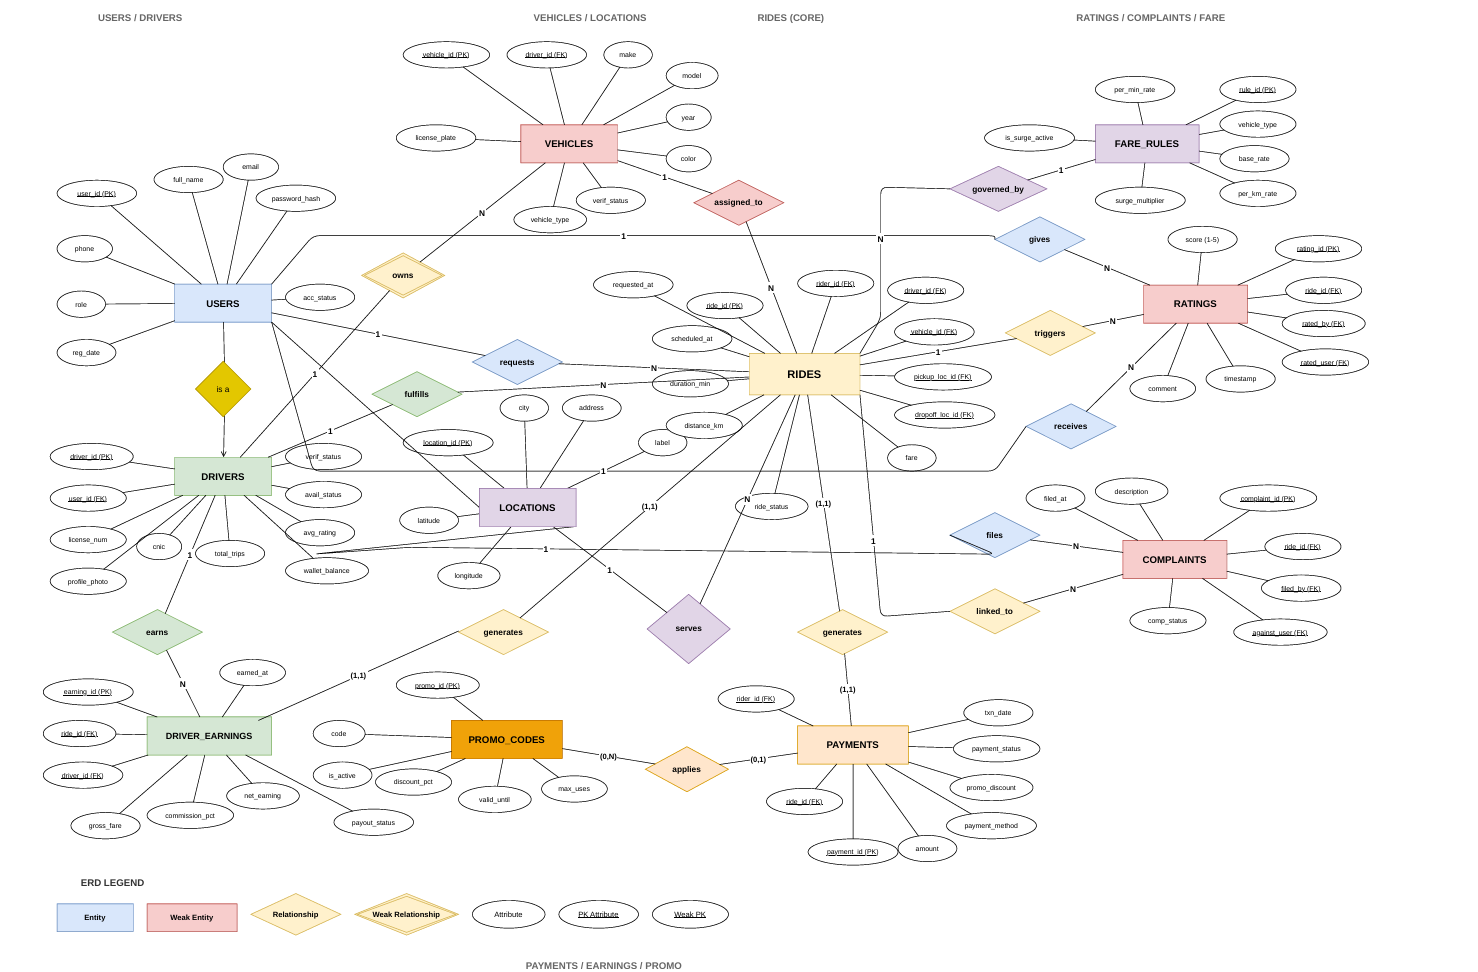
\includegraphics[width=\textwidth]{images/erd_diagram.png}
    \caption{Entity-Relationship Diagram for RideFlow Database}
    \label{fig:erd}
\end{figure}

The ER diagram in Figure \ref{fig:erd} illustrates the relationships between all entities in the RideFlow system. Key entities include Users, Riders, Drivers, Rides, Vehicles, Payments, and Locations.

\section{Database Schema Design}

\subsection{Core Tables}

\begin{longtable}{|p{3cm}|p{4cm}|p{6cm}|}
\caption{Database Schema Overview}
\label{tab:schema}\\
\hline
\textbf{Table Name} & \textbf{Primary Key} & \textbf{Description} \\
\hline
\endfirsthead
\hline
\textbf{Table Name} & \textbf{Primary Key} & \textbf{Description} \\
\hline
\endhead
users & user\_id & Stores all user credentials and basic info \\
\hline
riders & rider\_id & Extended profile for riders \\
\hline
drivers & driver\_id & Driver-specific information including license \\
\hline
vehicles & vehicle\_id & Vehicle details linked to drivers \\
\hline
rides & ride\_id & Core ride booking information \\
\hline
locations & location\_id & Geographic location data \\
\hline
payments & payment\_id & Payment transaction records \\
\hline
ratings & rating\_id & Driver and ride ratings \\
\hline
fare\_rules & rule\_id & Dynamic pricing configuration \\
\hline
promo\_codes & promo\_id & Promotional code management \\
\hline
\end{longtable}

\subsection{Relational Schema}

\begin{figure}[H]
    \centering
    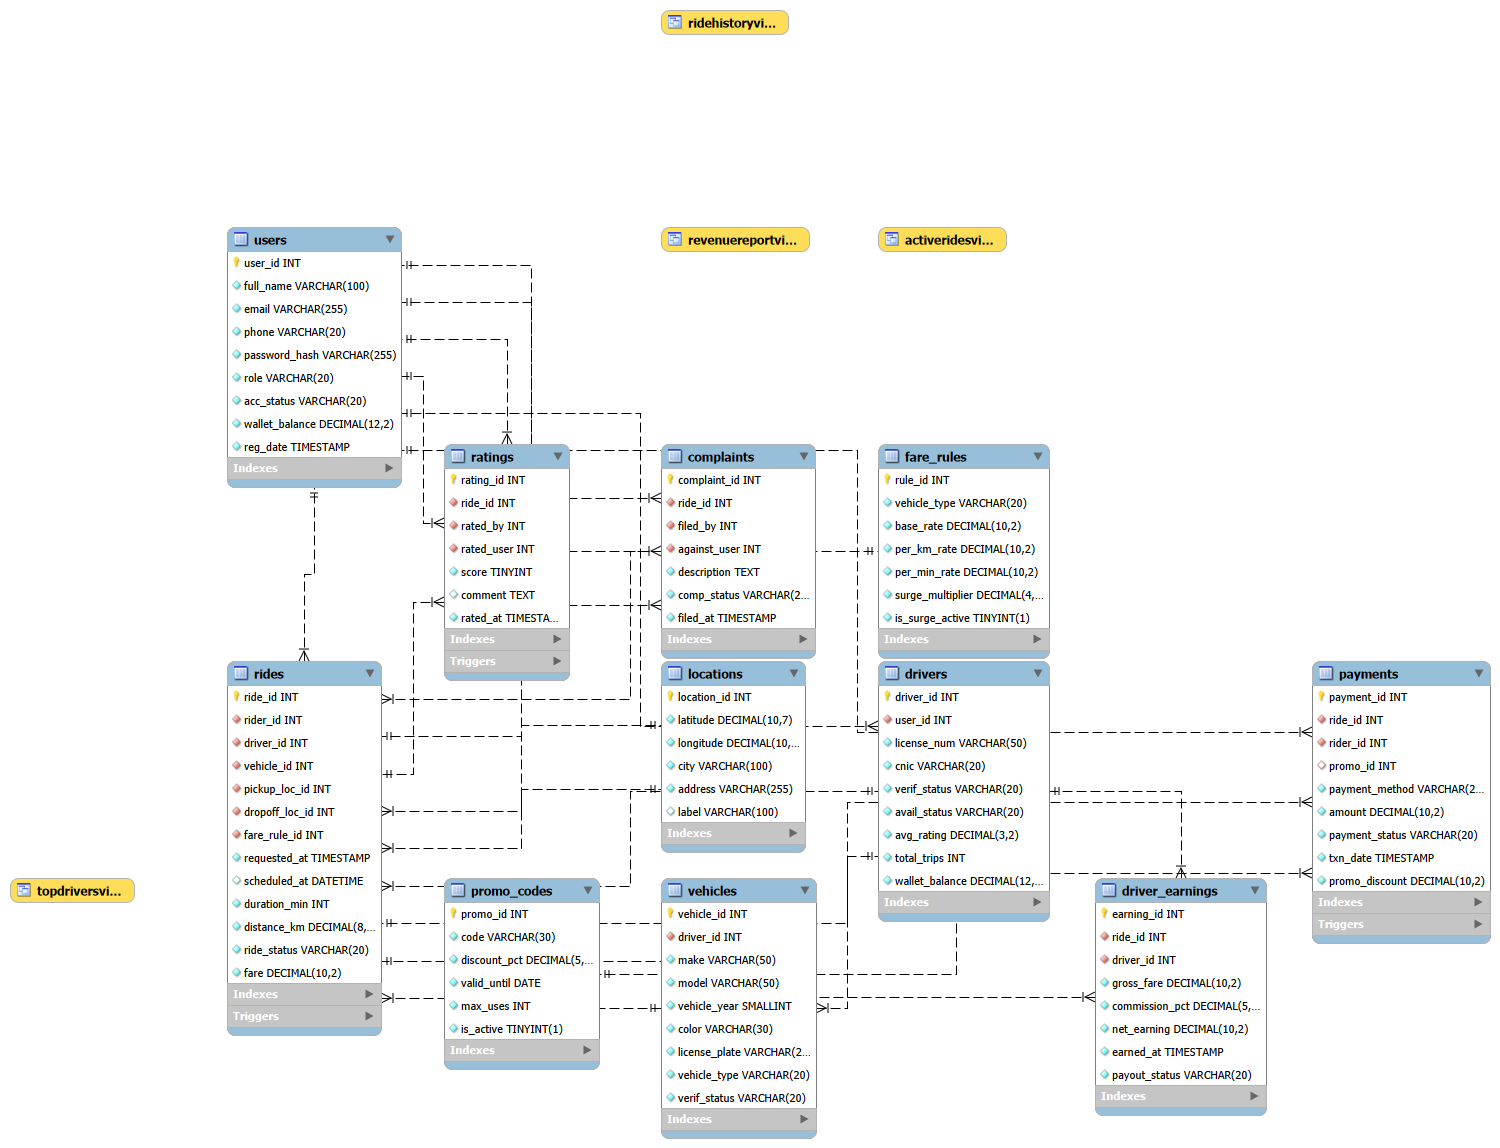
\includegraphics[width=0.9\textwidth]{images/relational_schema.png}
    \caption{Relational Schema with All Tables and Relationships}
    \label{fig:relational}
\end{figure}

\section{System Architecture}

\begin{figure}[H]
    \centering
    \includegraphics[width=0.8\textwidth]{images/system_architecture.png}
    \caption{Three-Tier Architecture of RideFlow}
    \label{fig:architecture}
\end{figure}

The system follows a three-tier architecture:
\begin{enumerate}
    \item \textbf{Presentation Layer}: HTML/CSS/JavaScript frontend
    \item \textbf{Application Layer}: Node.js/Express.js backend
    \item \textbf{Data Layer}: MySQL database with advanced SQL features
\end{enumerate}

% ==================== CHAPTER 3: DATABASE IMPLEMENTATION ====================
\chapter{Database Implementation}

\section{Basic SQL Queries}

\subsection{Query Examples}

\begin{lstlisting}[language=SQL, caption={List all completed rides for a specific rider}]
SELECT r.ride_id, r.requested_at, r.status, 
       r.pickup_address, r.dropoff_address, r.fare_amount
FROM rides r
WHERE r.rider_id = 1 
  AND r.status = 'Completed'
ORDER BY r.requested_at DESC;
\end{lstlisting}

\begin{lstlisting}[language=SQL, caption={List all drivers in a city ordered by rating}]
SELECT d.driver_id, u.full_name, d.avg_rating, 
       d.total_trips, l.city
FROM drivers d
JOIN users u ON d.user_id = u.user_id
JOIN locations l ON d.current_loc_id = l.location_id
WHERE l.city = 'Islamabad'
ORDER BY d.avg_rating DESC;
\end{lstlisting}

\section{Aggregate Functions and HAVING Clause}

\subsection{Revenue Calculation}

\begin{lstlisting}[language=SQL, caption={Calculate total revenue per city}]
SELECT l.city, 
       SUM(r.fare_amount) as total_revenue,
       COUNT(r.ride_id) as total_rides,
       AVG(r.fare_amount) as avg_fare
FROM rides r
JOIN locations l ON r.dropoff_loc_id = l.location_id
WHERE r.status = 'Completed'
GROUP BY l.city
HAVING total_revenue > 5000
ORDER BY total_revenue DESC;
\end{lstlisting}

\subsection{Driver Performance Analysis}

\begin{lstlisting}[language=SQL, caption={Drivers with low ratings requiring attention}]
SELECT d.driver_id, u.full_name, 
       AVG(rat.score) as avg_rating,
       COUNT(DISTINCT ri.ride_id) as total_rides
FROM drivers d
JOIN users u ON d.user_id = u.user_id
LEFT JOIN rides ri ON d.driver_id = ri.driver_id
LEFT JOIN ratings rat ON ri.ride_id = rat.ride_id
GROUP BY d.driver_id
HAVING avg_rating < 3.5 OR avg_rating IS NULL;
\end{lstlisting}

\section{Joins for Complex Reports}

\subsection{Multi-Table Trip Report}

\begin{lstlisting}[language=SQL, caption={Complete trip report with all details}]
SELECT r.ride_id,
       ru.full_name as rider_name,
       du.full_name as driver_name,
       v.vehicle_type, v.plate_num,
       r.pickup_address, r.dropoff_address,
       r.fare_amount, r.status
FROM rides r
INNER JOIN riders ri ON r.rider_id = ri.rider_id
INNER JOIN users ru ON ri.user_id = ru.user_id
LEFT JOIN drivers d ON r.driver_id = d.driver_id
LEFT JOIN users du ON d.user_id = du.user_id
LEFT JOIN vehicles v ON r.vehicle_id = v.vehicle_id
WHERE r.requested_at >= DATE_SUB(NOW(), INTERVAL 30 DAY);
\end{lstlisting}

\section{Views Implementation}

\subsection{Active Rides View}

\begin{lstlisting}[language=SQL, caption={ActiveRidesView - Real-time monitoring}]
CREATE VIEW ActiveRidesView AS
SELECT r.ride_id, r.status,
       ru.full_name as rider_name, ru.phone as rider_phone,
       du.full_name as driver_name, du.phone as driver_phone,
       v.vehicle_type, v.plate_num,
       r.pickup_address, r.dropoff_address,
       r.requested_at, r.fare_amount
FROM rides r
JOIN riders ri ON r.rider_id = ri.rider_id
JOIN users ru ON ri.user_id = ru.user_id
LEFT JOIN drivers d ON r.driver_id = d.driver_id
LEFT JOIN users du ON d.user_id = du.user_id
LEFT JOIN vehicles v ON r.vehicle_id = v.vehicle_id
WHERE r.status IN ('Requested', 'Accepted', 'In Progress');
\end{lstlisting}

\section{Indexes for Performance}

\begin{lstlisting}[language=SQL, caption={Performance optimization indexes}]
-- Index on rides for faster rider lookups
CREATE INDEX idx_rides_rider_id ON rides(rider_id);

-- Index for driver ride history
CREATE INDEX idx_rides_driver_id ON rides(driver_id);

-- Index for status-based queries
CREATE INDEX idx_rides_status ON rides(status);

-- Composite index for location-based searches
CREATE INDEX idx_locations_city ON locations(city);
\end{lstlisting}

\section{Stored Procedures}

\subsection{Fare Calculation Procedure}

\begin{lstlisting}[language=SQL, caption={CalculateFare procedure with surge pricing}]
DELIMITER //
CREATE PROCEDURE CalculateFare(
    IN p_distance_km DECIMAL(5,2),
    IN p_duration_min INT,
    IN p_vehicle_type ENUM('ECONOMY', 'PREMIUM', 'BIKE'),
    IN p_is_peak BOOLEAN,
    OUT p_total_fare DECIMAL(10,2),
    OUT p_base_fare DECIMAL(10,2),
    OUT p_surge_multiplier DECIMAL(3,2)
)
BEGIN
    DECLARE v_base_rate DECIMAL(10,2);
    DECLARE v_per_km_rate DECIMAL(5,2);
    DECLARE v_per_min_rate DECIMAL(5,2);
    
    -- Get fare rules
    SELECT base_rate, per_km_rate, per_min_rate
    INTO v_base_rate, v_per_km_rate, v_per_min_rate
    FROM fare_rules
    WHERE vehicle_type = p_vehicle_type;
    
    -- Calculate base fare
    SET p_base_fare = v_base_rate + 
                      (v_per_km_rate * p_distance_km) + 
                      (v_per_min_rate * p_duration_min);
    
    -- Apply surge if peak hour
    IF p_is_peak THEN
        SET p_surge_multiplier = 1.5;
    ELSE
        SET p_surge_multiplier = 1.0;
    END IF;
    
    SET p_total_fare = p_base_fare * p_surge_multiplier;
END //
DELIMITER ;
\end{lstlisting}

\section{Triggers}

\subsection{Payment Status Trigger}

\begin{lstlisting}[language=SQL, caption={Auto-update ride status on payment}]
DELIMITER //
CREATE TRIGGER trg_after_payment_paid
AFTER UPDATE ON payments
FOR EACH ROW
BEGIN
    IF NEW.payment_status = 'Paid' AND OLD.payment_status != 'Paid' THEN
        UPDATE rides 
        SET status = 'Completed', 
            completed_at = NOW()
        WHERE ride_id = NEW.ride_id;
    END IF;
END //
DELIMITER ;
\end{lstlisting}

\section{Events}

\subsection{Promo Code Expiry Event}

\begin{lstlisting}[language=SQL, caption={Midnight promo code cleanup}]
DELIMITER //
CREATE EVENT evt_expire_promo_codes
ON SCHEDULE EVERY 1 DAY
STARTS CURRENT_DATE + INTERVAL 1 DAY
DO
BEGIN
    UPDATE promo_codes 
    SET is_active = FALSE 
    WHERE valid_until < NOW() 
      AND is_active = TRUE;
END //
DELIMITER ;
\end{lstlisting}

\section{Data Control Language (DCL)}

\subsection{Role-Based Access Control}

\begin{lstlisting}[language=SQL, caption={Creating and granting roles}]
-- Create roles
CREATE ROLE admin_role, driver_role, rider_role, support_role;

-- Grant privileges to admin_role
GRANT ALL PRIVILEGES ON rideflow_db.* TO admin_role;

-- Grant limited privileges to driver_role
GRANT SELECT ON rideflow_db.rides TO driver_role;
GRANT SELECT ON rideflow_db.driver_earnings TO driver_role;
GRANT UPDATE (avail_status) ON rideflow_db.drivers TO driver_role;

-- Create user and assign role
CREATE USER 'app_driver'@'localhost' IDENTIFIED BY 'password';
GRANT driver_role TO 'app_driver'@'localhost';
FLUSH PRIVILEGES;
\end{lstlisting}

% ==================== CHAPTER 4: APPLICATION DEVELOPMENT ====================
\chapter{Application Development}

\section{Technology Stack}

\begin{table}[H]
\centering
\caption{Technology Stack}
\begin{tabular}{|l|l|l|}
\hline
\textbf{Layer} & \textbf{Technology} & \textbf{Purpose} \\
\hline
Backend & Node.js + Express.js & Server-side logic \\
Database & MySQL 8.0 & Data storage \\
Frontend & HTML5 + CSS3 + JavaScript & User interface \\
Authentication & bcryptjs + express-session & Security \\
Maps & Google Maps API & Location services \\
\hline
\end{tabular}
\end{table}

\section{Backend Architecture}

\subsection{Server.js Structure}

\begin{lstlisting}[language=JavaScript, caption={Express server setup}]
const express = require('express');
const mysql = require('mysql2/promise');
const bcrypt = require('bcryptjs');
const session = require('express-session');

const app = express();
const pool = mysql.createPool(dbConfig);

// Middleware
app.use(express.json());
app.use(express.static('public'));
app.use(session({
    secret: process.env.SESSION_SECRET,
    resave: false,
    saveUninitialized: false
}));
\end{lstlisting}

\subsection{API Endpoints}

\begin{longtable}{|p{4cm}|p{2cm}|p{6cm}|}
\caption{REST API Endpoints}
\label{tab:api}\\
\hline
\textbf{Endpoint} & \textbf{Method} & \textbf{Description} \\
\hline
\endfirsthead
/api/login & POST & User authentication \\
\hline
/api/rider/book & POST & Create new ride booking \\
\hline
/api/driver/toggle-status & POST & Change driver availability \\
\hline
/api/driver/accept-ride & POST & Accept ride request \\
\hline
/api/admin/stats & GET & Dashboard statistics \\
\hline
/api/admin/active-rides & GET & Live ride monitoring \\
\hline
\end{longtable}

\section{Frontend Implementation}

\subsection{Responsive Design}

\begin{figure}[H]
    \centering
    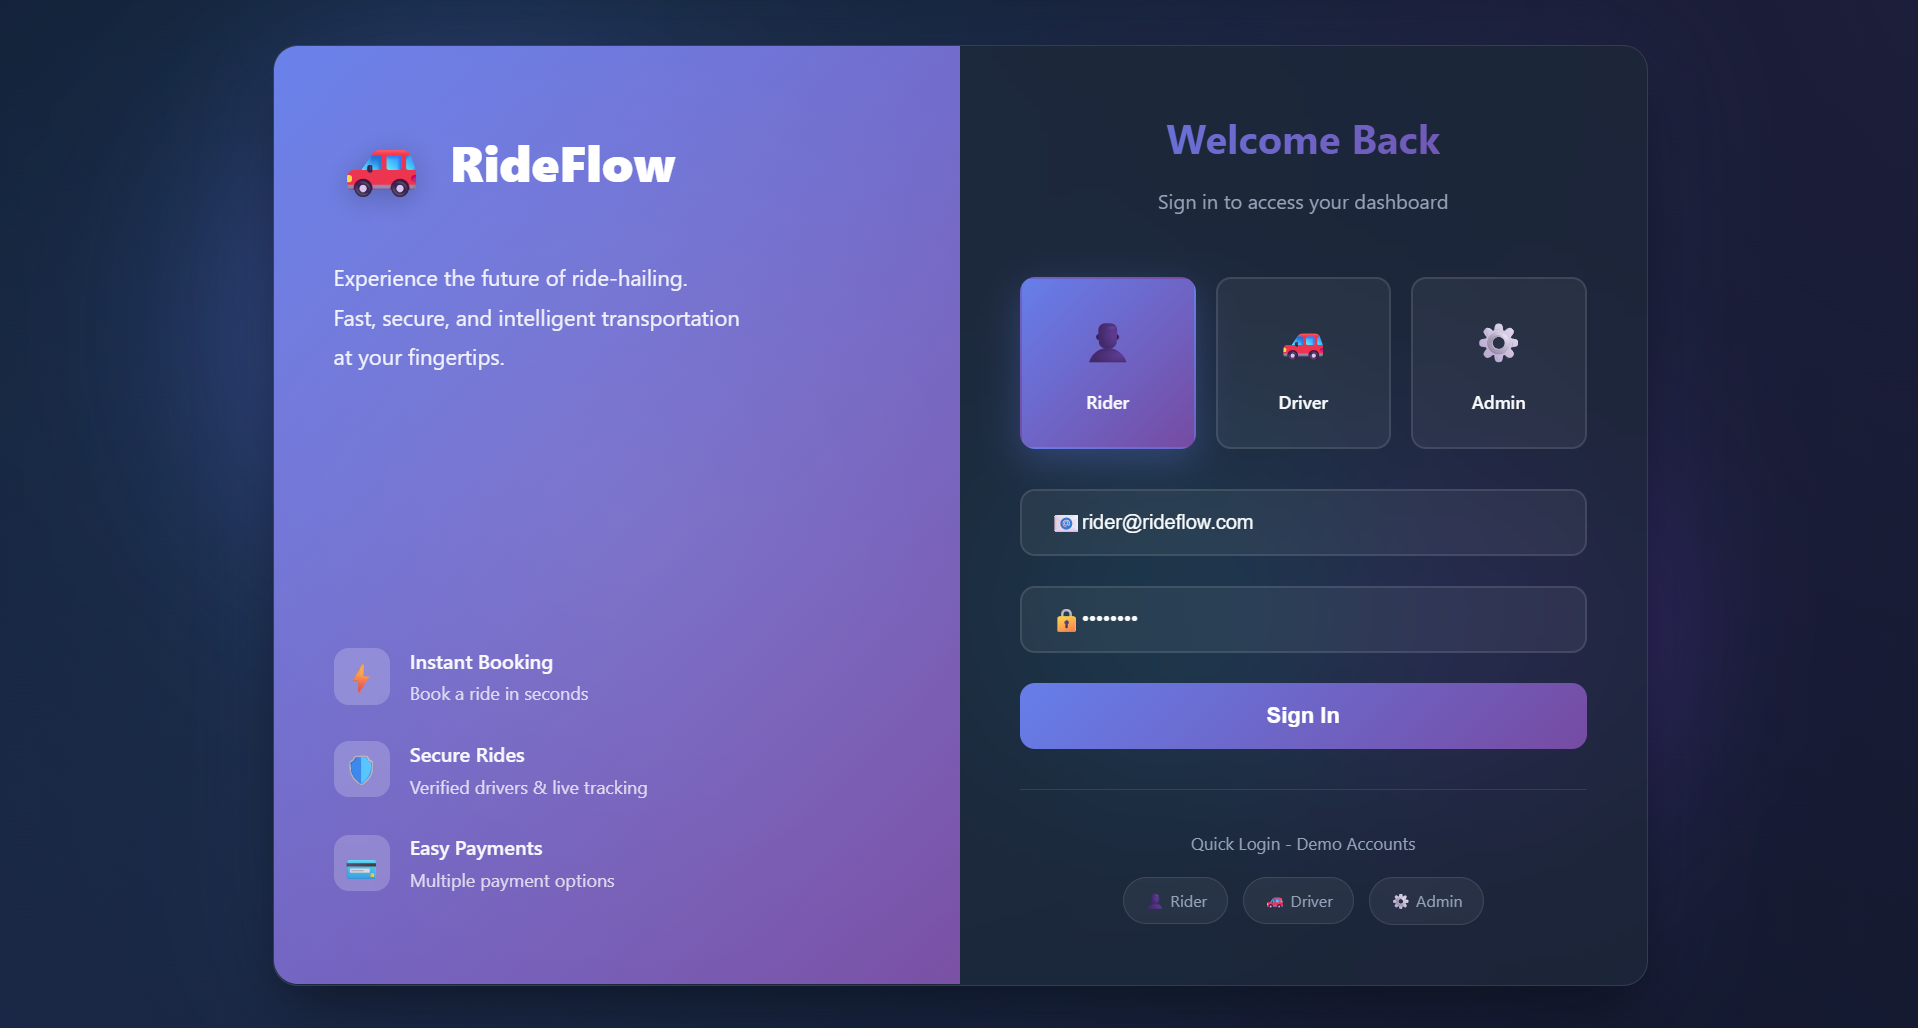
\includegraphics[width=\textwidth]{images/login_page.png}
    \caption{Login Page - Entry point for all users}
    \label{fig:login}
\end{figure}

\subsection{Rider Dashboard}

\begin{figure}[H]
    \centering
    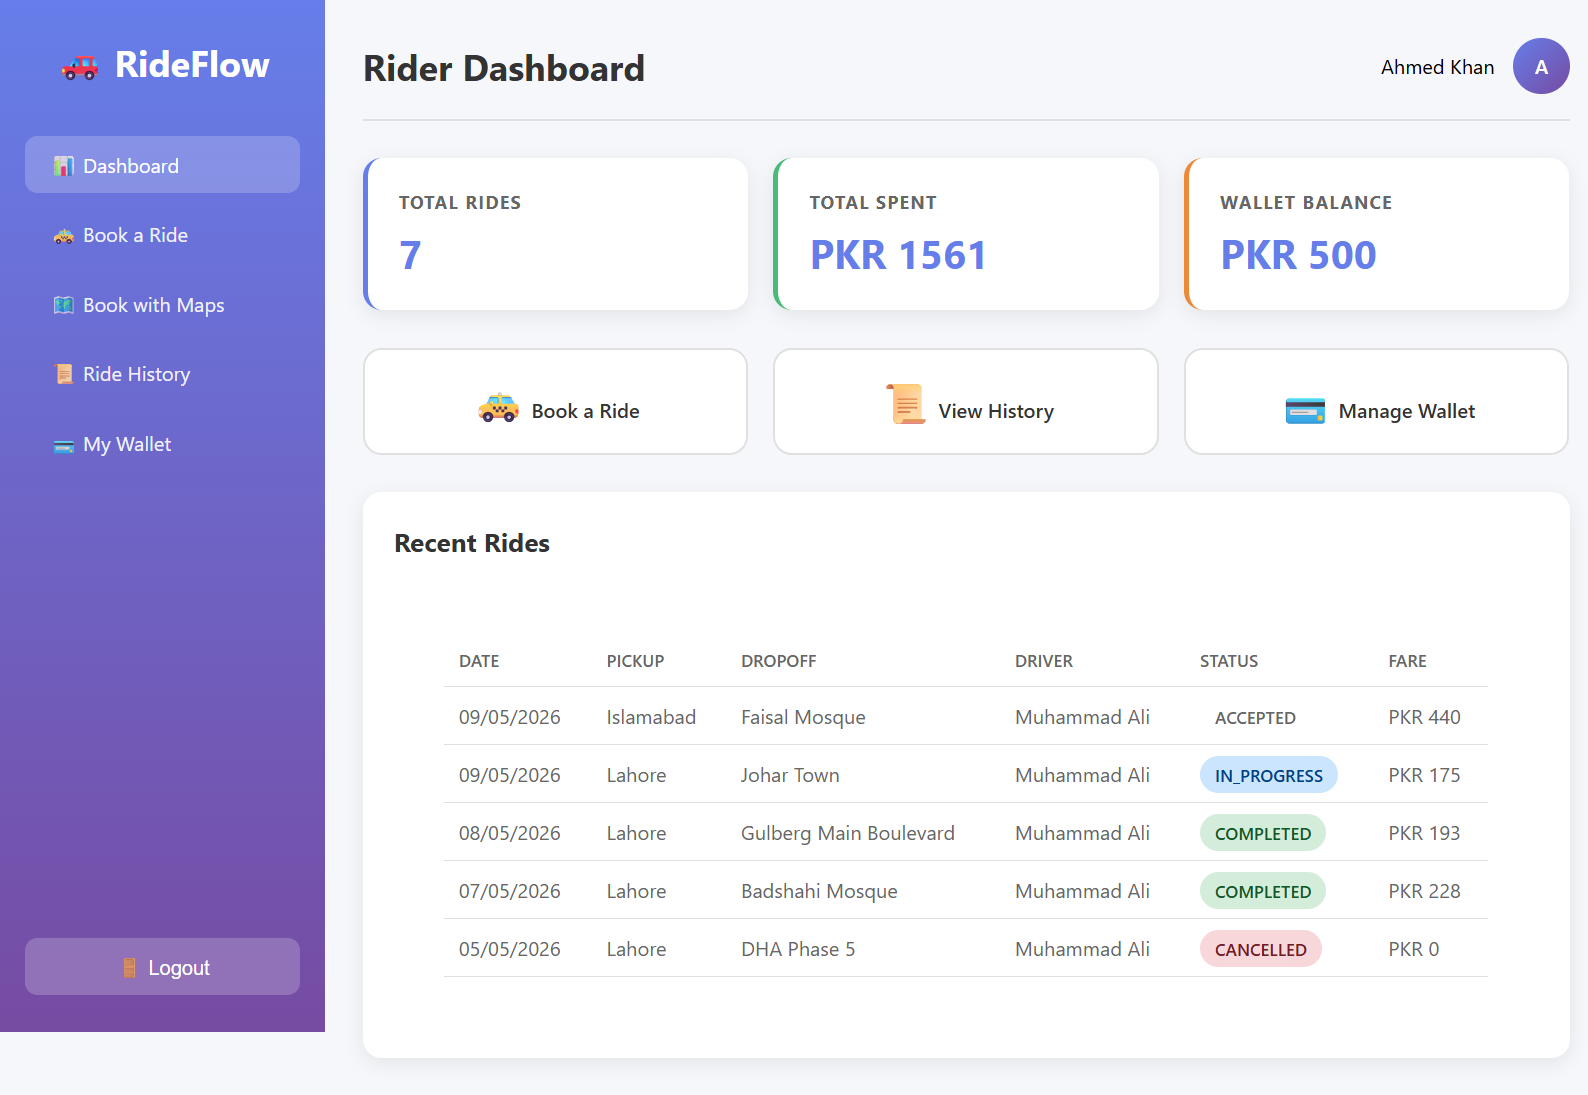
\includegraphics[width=\textwidth]{images/rider_dashboard.png}
    \caption{Rider Dashboard - Main interface for ride booking}
    \label{fig:rider-dash}
\end{figure}

\subsection{Book with Maps Feature}

\begin{figure}[H]
    \centering
    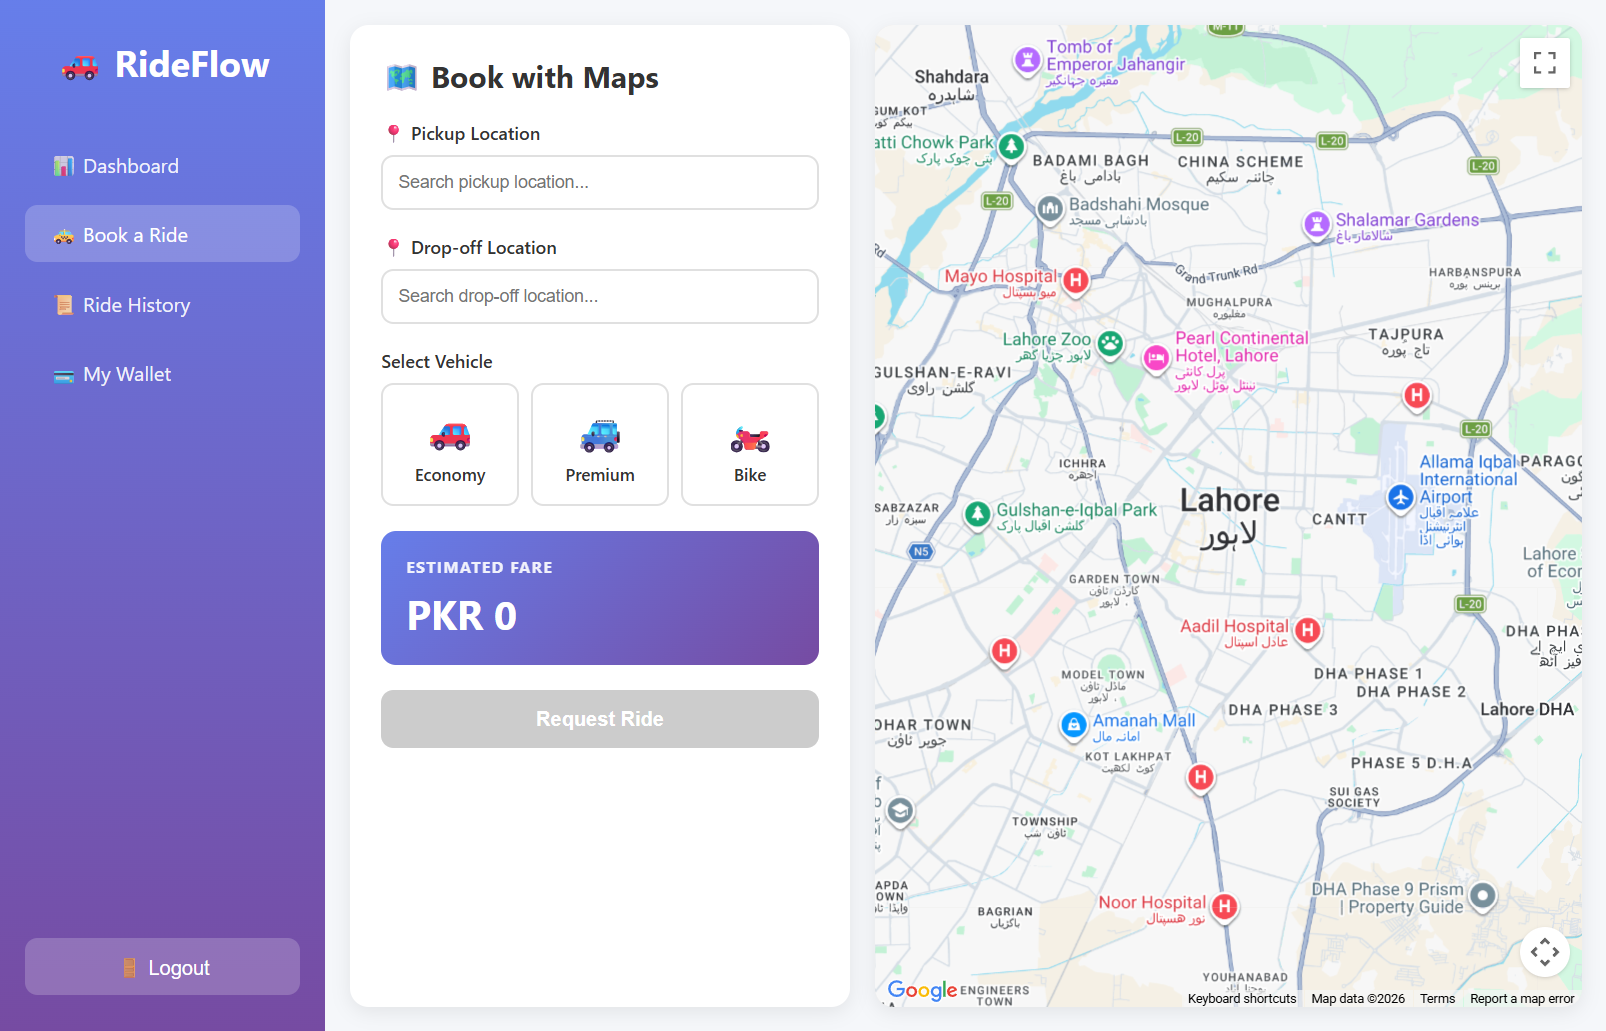
\includegraphics[width=\textwidth]{images/book_with_maps.png}
    \caption{Google Maps Integration - Interactive ride booking}
    \label{fig:maps}
\end{figure}

\subsection{Driver Dashboard}

\begin{figure}[H]
    \centering
    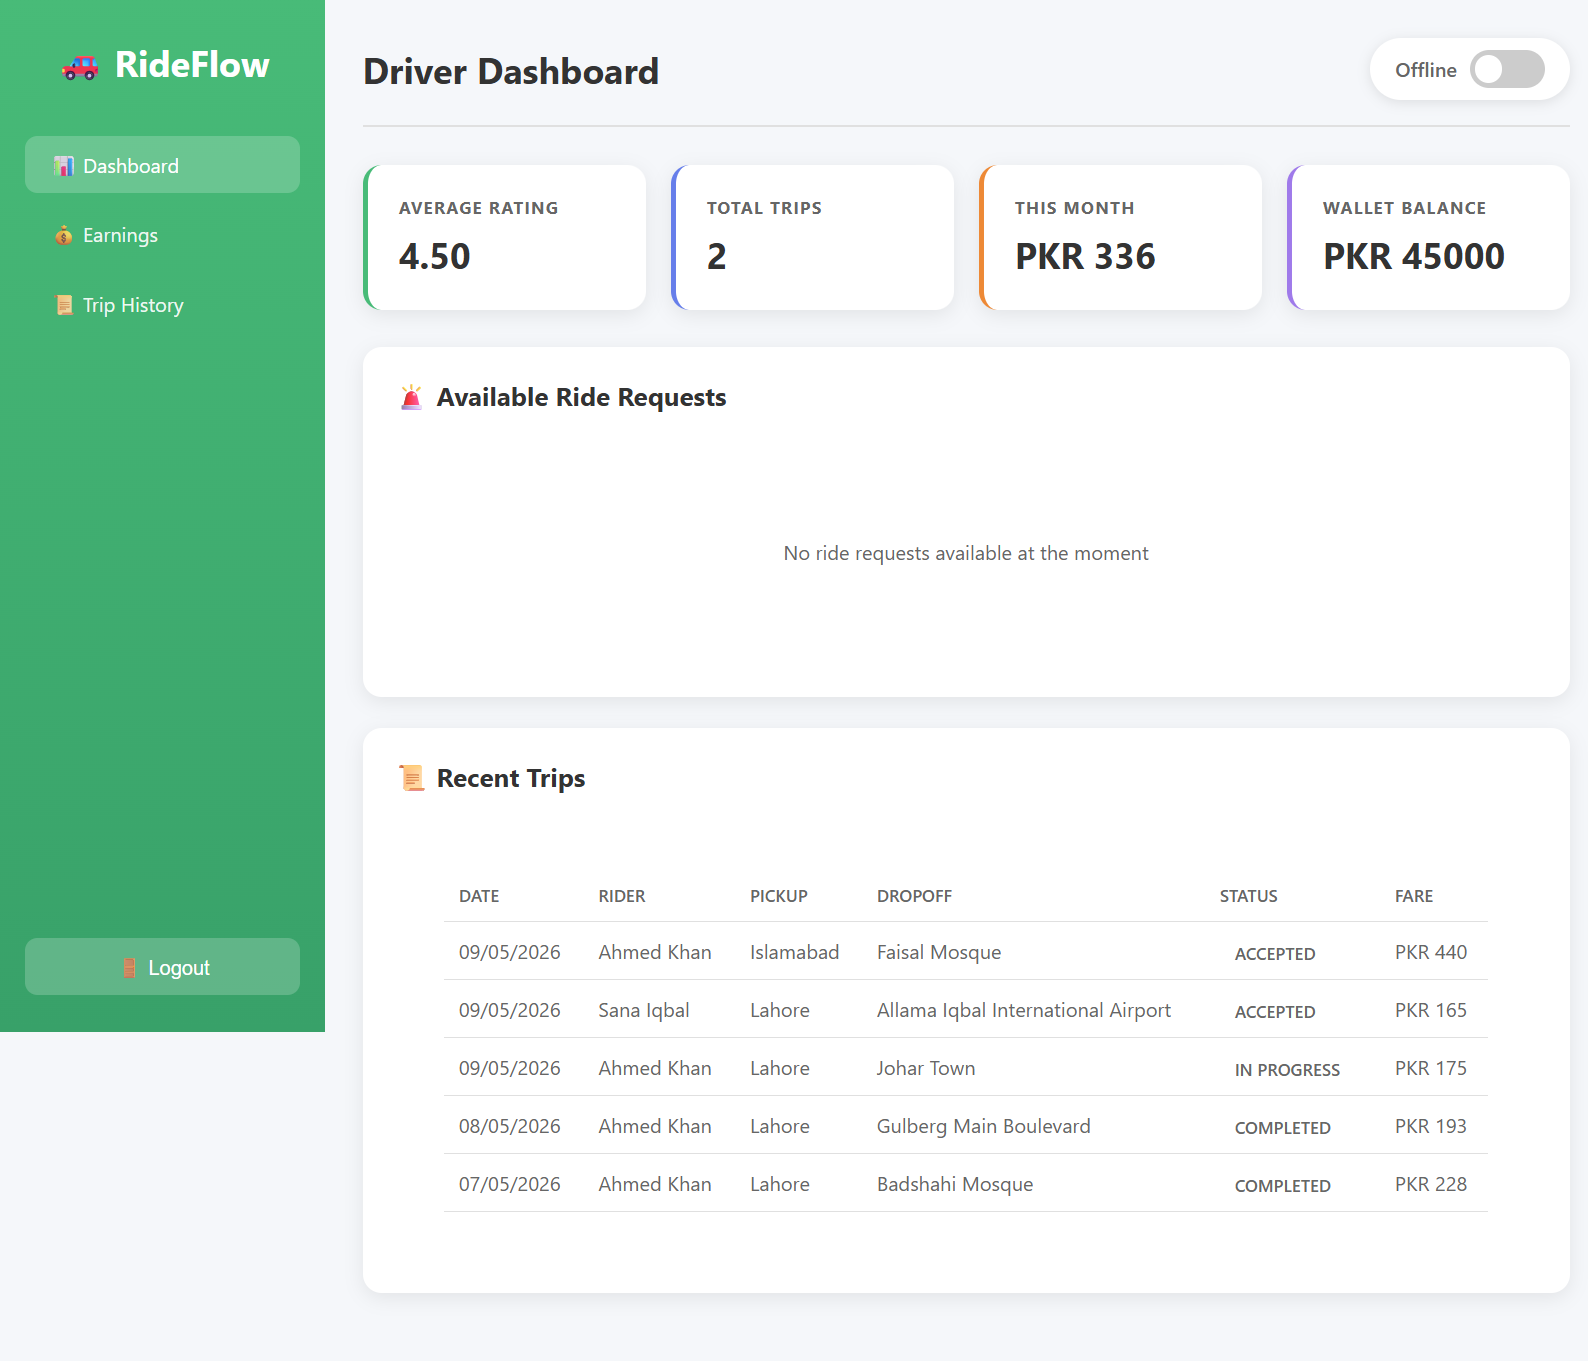
\includegraphics[width=\textwidth]{images/driver_dashboard.png}
    \caption{Driver Dashboard - Ride acceptance and earnings}
    \label{fig:driver-dash}
\end{figure}

\subsection{Admin Panel}

\begin{figure}[H]
    \centering
    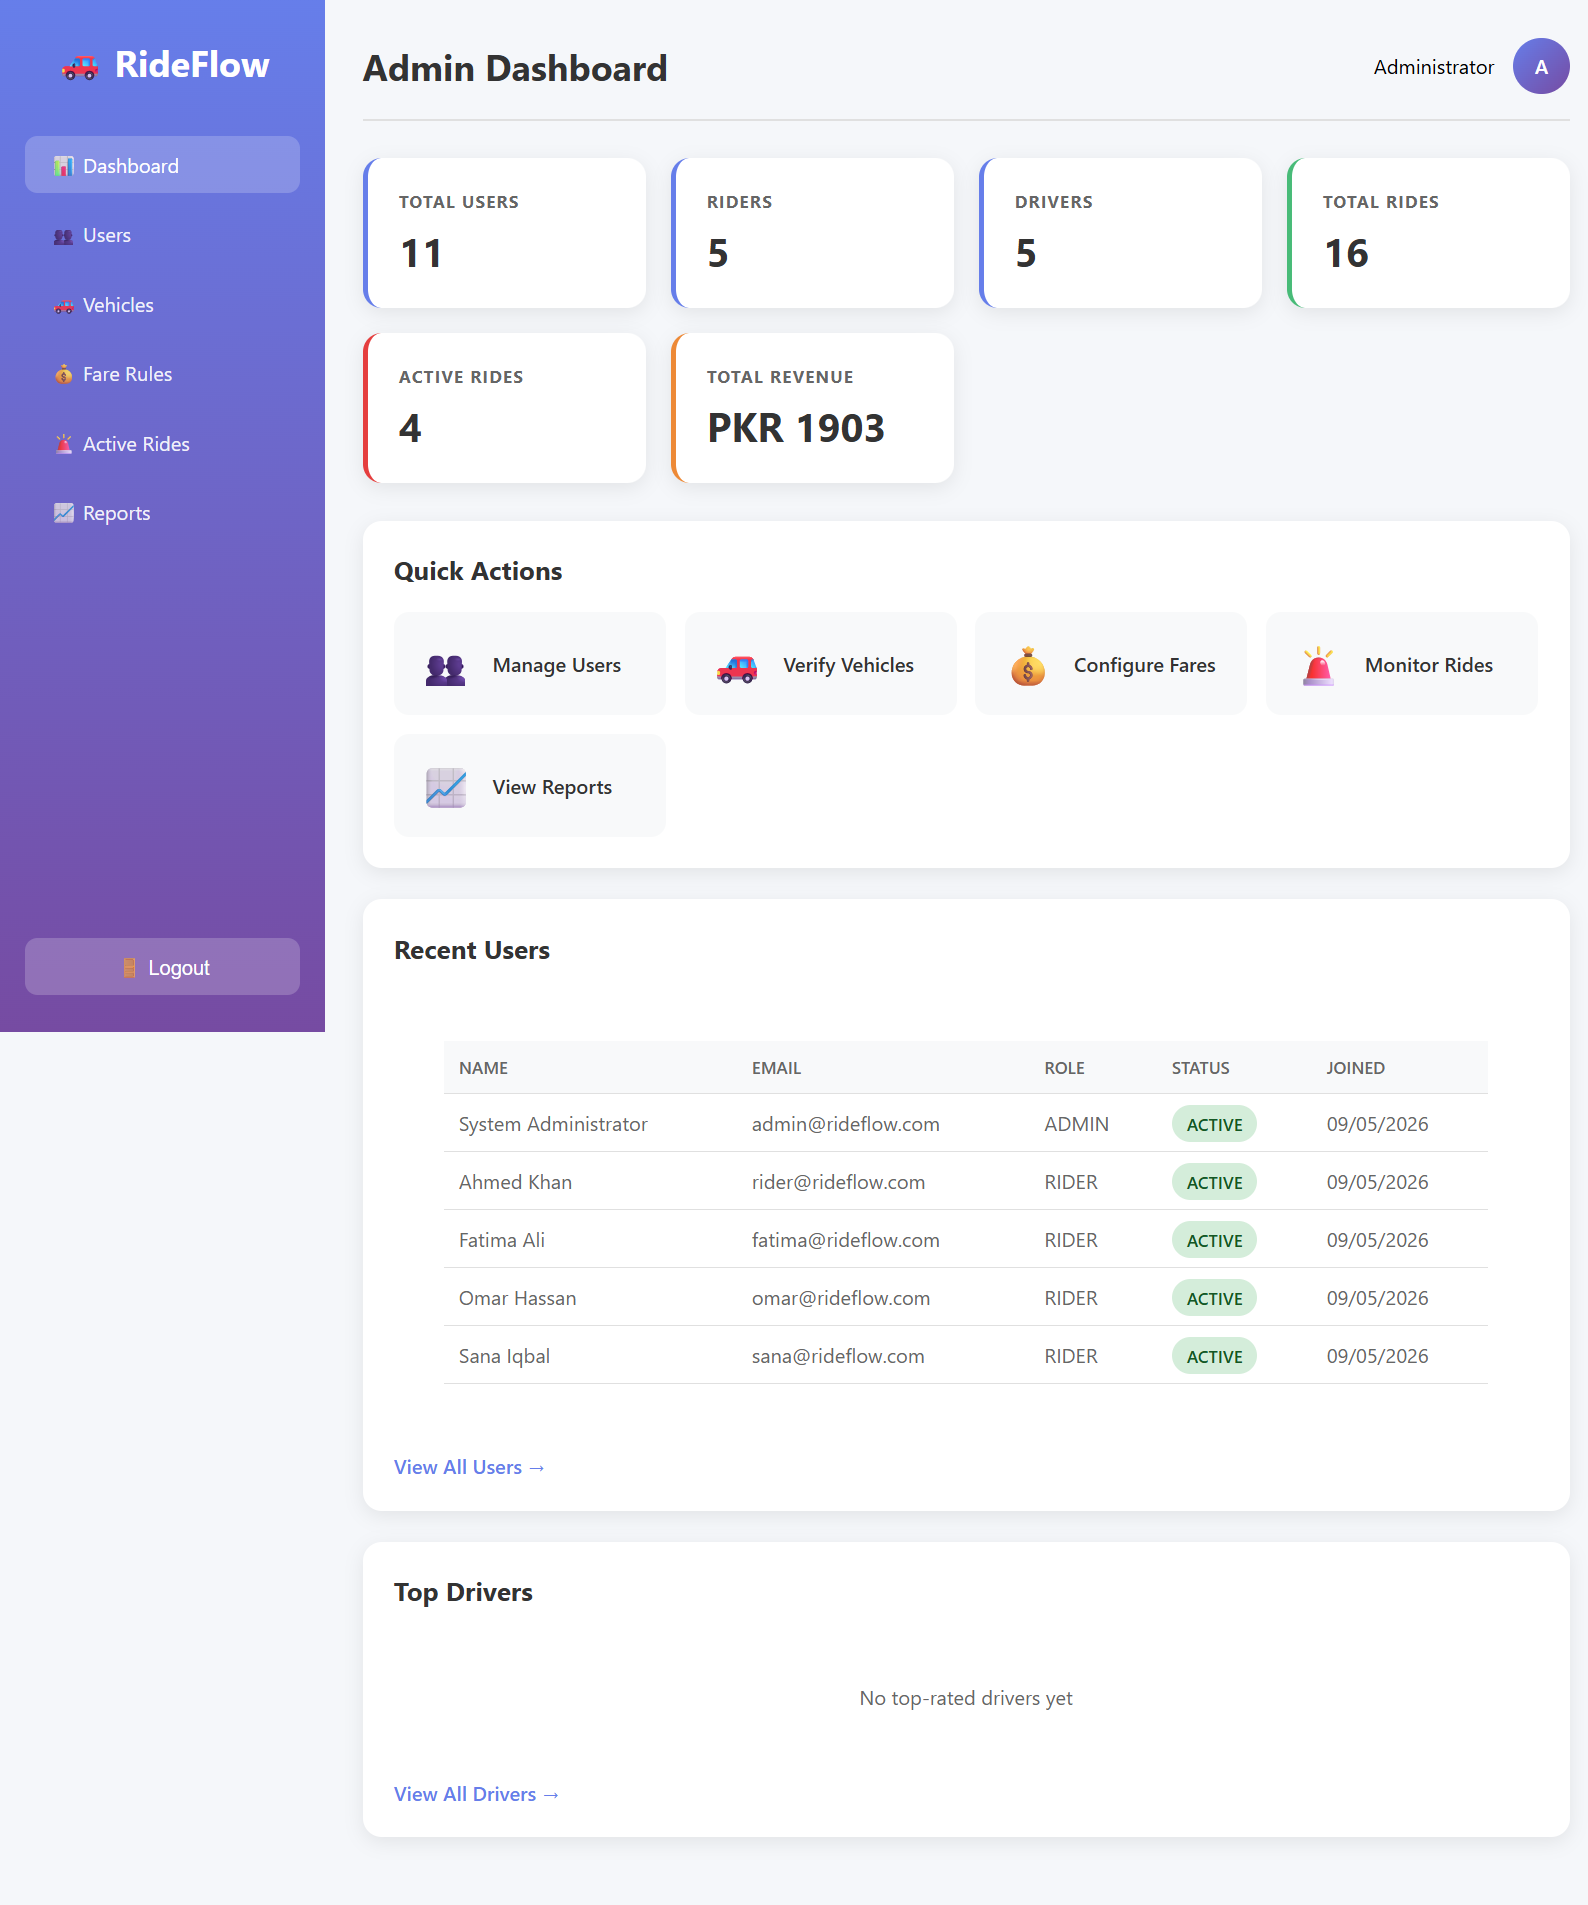
\includegraphics[width=\textwidth]{images/admin_dashboard.png}
    \caption{Admin Dashboard - System overview and analytics}
    \label{fig:admin-dash}
\end{figure}

\begin{figure}[H]
    \centering
    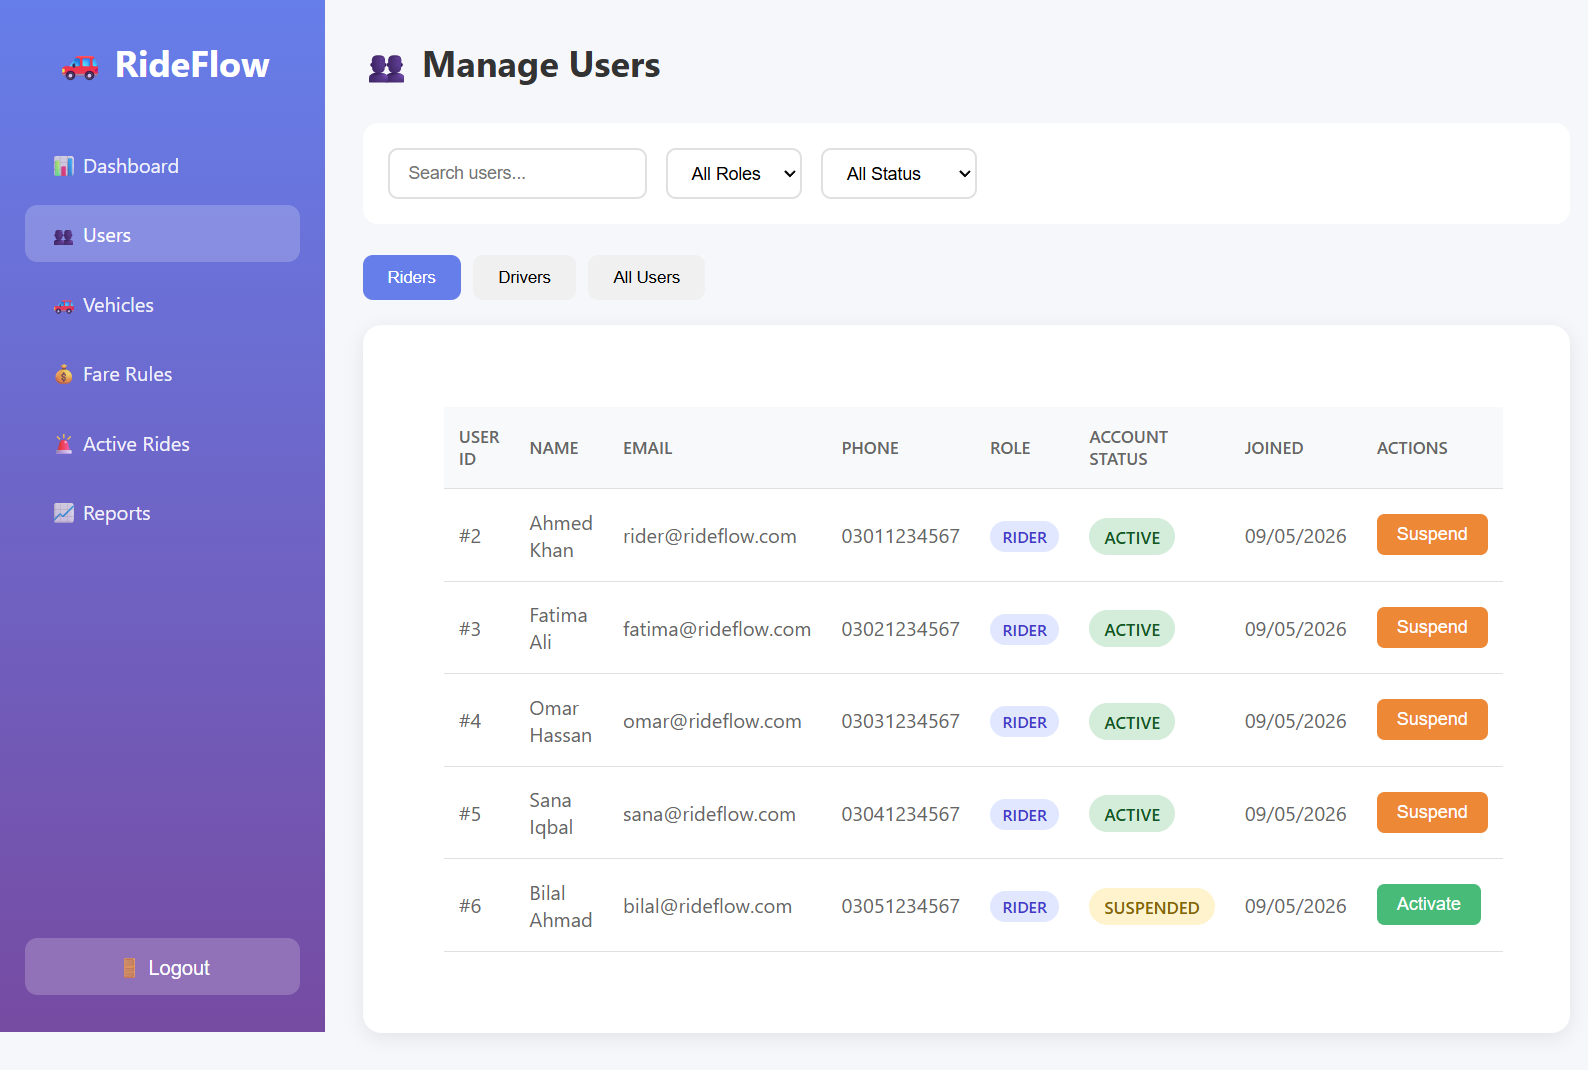
\includegraphics[width=\textwidth]{images/admin_users.png}
    \caption{User Management - Admin control panel}
    \label{fig:admin-users}
\end{figure}

% ==================== CHAPTER 5: FEATURES DEMONSTRATION ====================
\chapter{Features Demonstration}

\section{Core Features}

\subsection{Authentication System}
\begin{itemize}
    \item Role-based login (Rider, Driver, Admin)
    \item Session management with secure cookies
    \item Password hashing with bcrypt
\end{itemize}

\subsection{Rider Features}
\begin{enumerate}
    \item \textbf{Book a Ride}: Simple form-based booking
    \item \textbf{Book with Maps}: Google Maps integrated booking with:
    \begin{itemize}
        \item Location autocomplete
        \item Visual route display
        \item Real-time fare calculation
        \item Distance and time estimation
    \end{itemize}
    \item \textbf{Ride History}: Complete trip records
    \item \textbf{Wallet Management}: Balance tracking and history
\end{enumerate}

\subsection{Driver Features}
\begin{enumerate}
    \item \textbf{Availability Toggle}: Online/Offline status
    \item \textbf{Ride Requests}: Accept or reject rides
    \item \textbf{Earnings Dashboard}: Income tracking
    \item \textbf{Trip History}: Completed rides log
\end{enumerate}

\subsection{Admin Features}
\begin{enumerate}
    \item \textbf{User Management}: View, filter, suspend users
    \item \textbf{Vehicle Verification}: Approve/reject driver vehicles
    \item \textbf{Fare Rules}: Dynamic pricing configuration
    \item \textbf{Active Rides}: Real-time ride monitoring
    \item \textbf{Reports}: Revenue analytics and insights
\end{enumerate}

\section{Advanced Database Features in Action}

\subsection{Stored Procedure: Fare Calculation}

\begin{figure}[H]
    \centering
    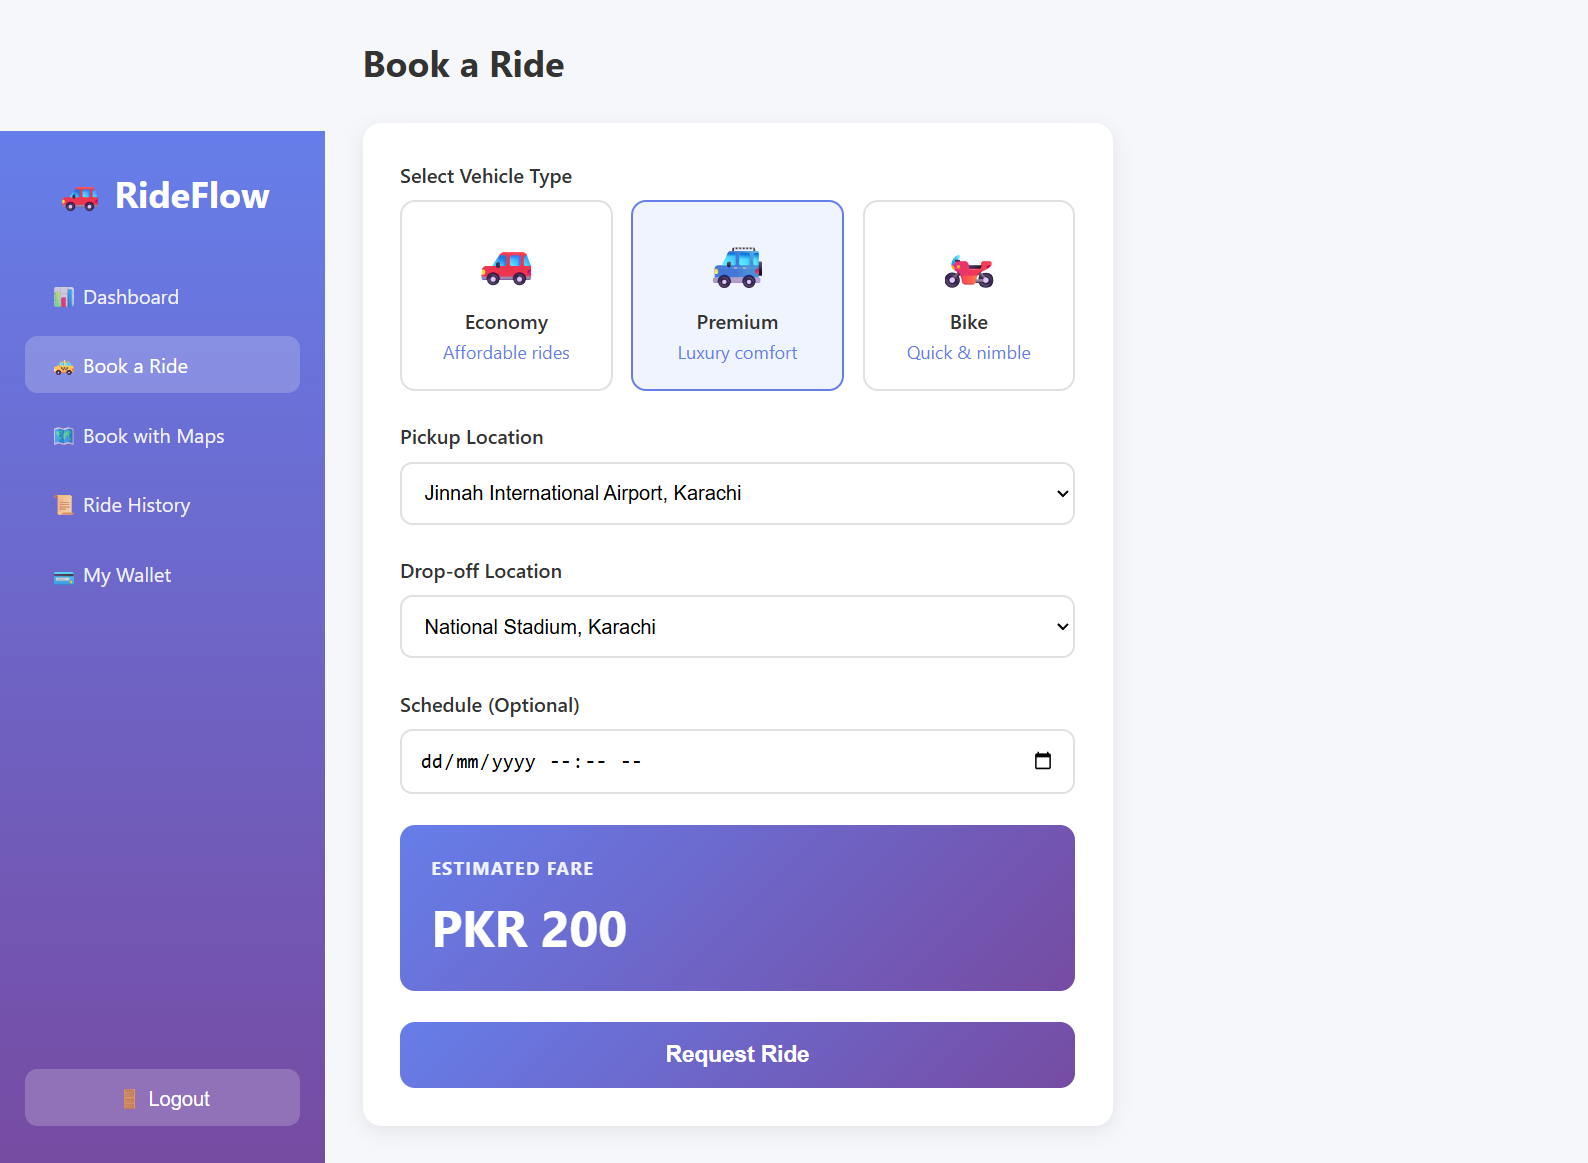
\includegraphics[width=0.8\textwidth]{images/fare_calculation.png}
    \caption{Dynamic fare calculation with surge pricing}
    \label{fig:fare}
\end{figure}

\subsection{Trigger: Auto-Complete Ride}

When a payment status changes to 'Paid', the trigger automatically updates the ride status to 'Completed'.

\subsection{Event: Promo Code Cleanup}

Every midnight, the event scheduler deactivates expired promotional codes.

\subsection{View: Active Rides Monitoring}

\begin{figure}[H]
    \centering
    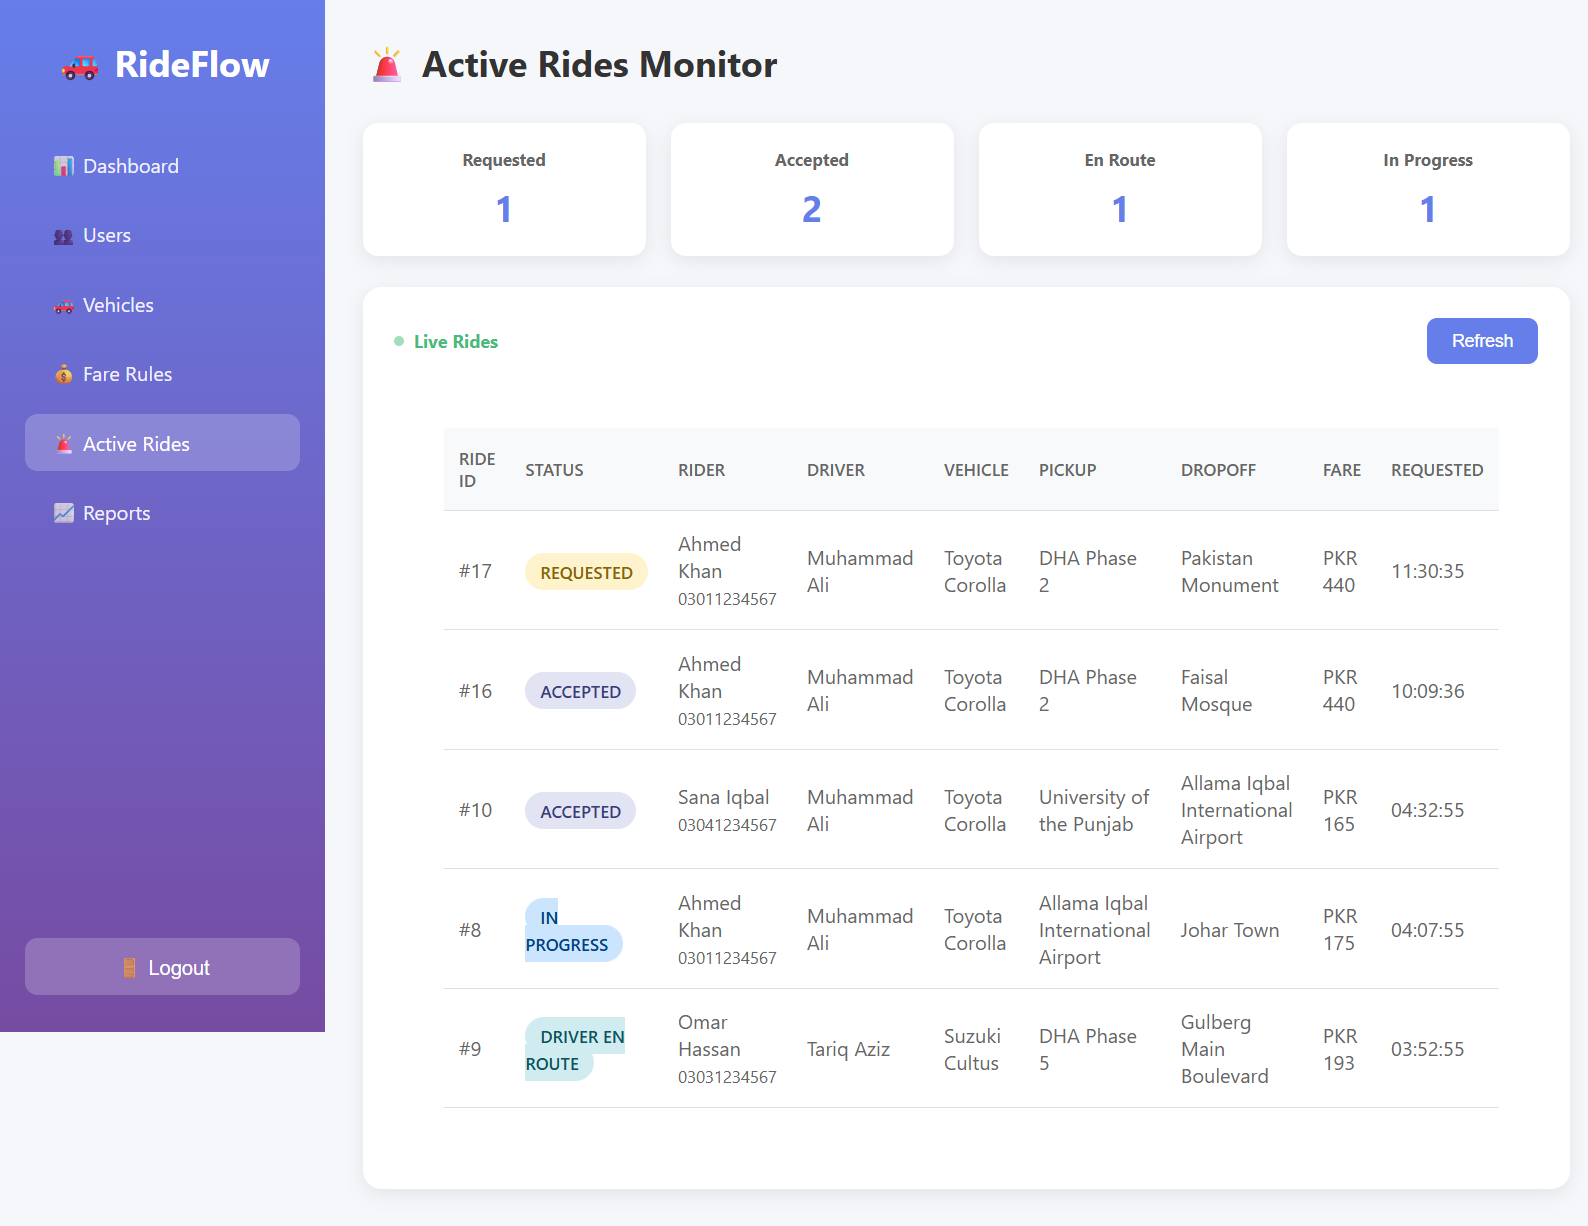
\includegraphics[width=\textwidth]{images/active_rides.png}
    \caption{Real-time active rides monitoring using ActiveRidesView}
    \label{fig:active}
\end{figure}

% ==================== CHAPTER 6: WORK DIVISION ====================
\chapter{Work Division}

\section{Group Member Responsibilities}

\begin{table}[H]
\centering
\caption{Work Division Between Group Members}
\begin{tabular}{|p{4cm}|p{5cm}|p{5cm}|}
\hline
\textbf{Component} & \textbf{Mohid Abbas (24I-0074)} & \textbf{Ubaid ur Rehman (24I-0022)} \\
\hline
\textbf{Database Design} & ER Diagram, Schema Design & Relationship mapping, Constraints \\
\hline
\textbf{SQL Implementation} & Views, Stored Procedures, Indexes & Triggers, Events, DCL, Queries \\
\hline
\textbf{Backend Development} & API endpoints, Authentication & Database connection, Session management \\
\hline
\textbf{Frontend Development} & Rider Dashboard, Admin Panel & Driver Dashboard, Login/Signup \\
\hline
\textbf{Google Maps} & Maps API integration & Location services, Geocoding \\
\hline
\textbf{Testing} & Unit testing, Integration testing & SQL testing, UI testing \\
\hline
\textbf{Documentation} & LaTeX Report, Code comments & README files, Setup guides \\
\hline
\textbf{Deployment} & Local deployment testing & Cloud deployment guides \\
\hline
\end{tabular}
\end{table}

\section{Contribution Percentage}

\begin{figure}[H]
    \centering
    \begin{tikzpicture}
        \pie[text=legend, radius=3]{
            50/Mohid Abbas (24I-0074),
            50/Ubaid ur Rehman (24I-0022)
        }
    \end{tikzpicture}
    \caption{Equal Contribution Distribution}
    \label{fig:contribution}
\end{figure}

Both group members contributed equally (50\% each) to the project.

% ==================== CHAPTER 7: TESTING ====================
\chapter{Testing and Validation}

\section{Testing Strategy}

\subsection{Database Testing}
\begin{itemize}
    \item SQL query execution validation
    \item Stored procedure output verification
    \item Trigger functionality testing
    \item Event scheduler verification
    \item Index performance analysis
\end{itemize}

\subsection{Application Testing}
\begin{itemize}
    \item Unit testing for API endpoints
    \item Integration testing for database operations
    \item UI/UX testing for all user roles
    \item Security testing for authentication
\end{itemize}

\section{Test Cases}

\begin{table}[H]
\centering
\caption{Sample Test Cases}
\begin{tabular}{|p{1cm}|p{4cm}|p{4cm}|p{3cm}|}
\hline
\textbf{ID} & \textbf{Test Case} & \textbf{Expected Result} & \textbf{Status} \\
\hline
TC01 & Rider books a ride & Ride created in database & Passed \\
\hline
TC02 & Driver accepts ride & Ride status changes to 'Accepted' & Passed \\
\hline
TC03 & Payment marked paid & Trigger updates ride to 'Completed' & Passed \\
\hline
TC04 & Calculate fare procedure & Correct fare with surge & Passed \\
\hline
TC05 & Admin views active rides & ActiveRidesView returns data & Passed \\
\hline
\end{tabular}
\end{table}

% ==================== CHAPTER 8: DEPLOYMENT ====================
\chapter{Deployment}

\section{Local Deployment}

\subsection{Prerequisites}
\begin{itemize}
    \item Node.js (v14 or higher)
    \item MySQL (v8.0 or higher)
    \item npm or yarn package manager
\end{itemize}

\subsection{Installation Steps}

\begin{lstlisting}[language=bash, caption={Setup commands}]
# 1. Database setup
mysql -u root -p
SOURCE rideflow_relational_schema.sql;
SOURCE rideflow_deliverable3_advanced_sql.sql;
SOURCE rideflow_seed_data.sql;

# 2. Application setup
cd app
npm install
copy .env.example .env
# Edit .env with your credentials

# 3. Start server
npm start
\end{lstlisting}

\section{Cloud Deployment Options}

\subsection{Render.com Deployment}
\begin{enumerate}
    \item Push code to GitHub
    \item Connect repository to Render
    \item Add environment variables
    \item Deploy automatically
\end{enumerate}

\subsection{Database Hosting}
\begin{itemize}
    \item PlanetScale: Free MySQL hosting
    \item Aiven: Free 5GB MySQL
    \item Railway: Simple deployment with database
\end{itemize}

% ==================== CHAPTER 9: CONCLUSION ====================
\chapter{Conclusion and Future Work}

\section{Project Summary}
RideFlow successfully demonstrates a complete ride-hailing platform implementing all required database concepts. The project includes:
\begin{itemize}
    \item Comprehensive database design with 10+ tables
    \item Advanced SQL features (views, procedures, triggers, events)
    \item Role-based access control
    \item Functional web application with three user roles
    \item Google Maps integration for location services
\end{itemize}

\section{Challenges Faced}
\begin{enumerate}
    \item Database relationship complexity - Solved through careful ER diagram design
    \item SQL syntax differences - Adapted for MySQL 8.0 compatibility
    \item Google Maps API integration - Implemented secure key storage
    \item Session management - Used express-session with proper configuration
\end{enumerate}

\section{Future Enhancements}
\begin{itemize}
    \item Real-time driver tracking with WebSockets
    \item Mobile application using React Native
    \item Payment gateway integration (Stripe/PayPal)
    \item AI-based route optimization
    \item Chat system between riders and drivers
    \item Push notifications
\end{itemize}

\section{Learning Outcomes}
\begin{itemize}
    \item Advanced SQL query writing
    \item Database design and normalization
    \item Stored procedures and triggers
    \item Role-based security implementation
    \item Full-stack web development
    \item Third-party API integration
\end{itemize}

% ==================== REFERENCES ====================
\chapter*{References}
\addcontentsline{toc}{chapter}{References}

\begin{enumerate}
    \item MySQL 8.0 Documentation - \url{https://dev.mysql.com/doc/}
    \item Express.js Guide - \url{https://expressjs.com/en/guide/routing.html}
    \item Google Maps Platform - \url{https://developers.google.com/maps}
    \item Database Systems: The Complete Book (Garcia-Molina, Ullman, Widom)
    \item W3Schools SQL Tutorial - \url{https://www.w3schools.com/sql/}
\end{enumerate}

% ==================== APPENDICES ====================
\appendix
\chapter{Complete File Structure}

\begin{lstlisting}[language=bash, basicstyle=\ttfamily\scriptsize]
RideFlow-DBMS/
|-- DELIVERABLE3_README.md
|-- DEPLOYMENT_GUIDE.md
|-- GOOGLE_MAPS_SETUP.md
|-- PROJECT_SUMMARY.md
|-- SECURITY_SUMMARY.md
|-- README.md
|-- rideflow_relational_schema.sql
|-- rideflow_deliverable3_advanced_sql.sql
|-- rideflow_seed_data.sql
|-- erd.drawio
|-- erd.drawio.pdf
|-- app/
|   |-- package.json
|   |-- server.js
|   |-- .env
|   |-- .env.example
|   |-- public/
|       |-- login.html
|       |-- rider/
|       |   |-- dashboard.html
|       |   |-- book.html
|       |   |-- book-with-maps.html
|       |   |-- history.html
|       |   |-- wallet.html
|       |-- driver/
|       |   |-- dashboard.html
|       |   |-- earnings.html
|       |   |-- history.html
|       |-- admin/
|           |-- dashboard.html
|           |-- users.html
|           |-- vehicles.html
|           |-- fare-rules.html
|           |-- active-rides.html
|           |-- reports.html
\end{lstlisting}

\chapter{SQL File Contents Summary}

\section{rideflow\_relational\_schema.sql}
Contains CREATE TABLE statements for all database tables including:
\begin{itemize}
    \item users, riders, drivers tables
    \item vehicles, rides, locations tables
    \item payments, ratings, fare\_rules tables
    \item promo\_codes, driver\_earnings tables
\end{itemize}

\section{rideflow\_deliverable3\_advanced\_sql.sql}
Contains all advanced SQL features organized in sections:
\begin{enumerate}
    \item Basic Queries (SELECT, WHERE, ORDER BY)
    \item Aggregate Functions (SUM, AVG, COUNT, HAVING)
    \item Joins for Reports (INNER, LEFT, multi-table)
    \item Views (4 views)
    \item Indexes (7 indexes)
    \item Stored Procedures (5 procedures)
    \item Triggers (5 triggers)
    \item Events (1 event)
    \item DCL (4 roles with GRANT/REVOKE)
\end{enumerate}

\chapter{Screenshots Index}

\begin{table}[H]
\centering
\caption{Required Screenshots for Report}
\begin{tabular}{|p{1cm}|p{6cm}|p{6cm}|}
\hline
\textbf{No.} & \textbf{Screenshot Description} & \textbf{File Name} \\
\hline
1 & FAST University Logo & images/fast\_logo.png \\
\hline
2 & ER Diagram & images/erd\_diagram.png \\
\hline
3 & Relational Schema & images/relational\_schema.png \\
\hline
4 & System Architecture & images/system\_architecture.png \\
\hline
5 & Login Page & images/login\_page.png \\
\hline
6 & Rider Dashboard & images/rider\_dashboard.png \\
\hline
7 & Book with Maps & images/book\_with\_maps.png \\
\hline
8 & Driver Dashboard & images/driver\_dashboard.png \\
\hline
9 & Admin Dashboard & images/admin\_dashboard.png \\
\hline
10 & User Management & images/admin\_users.png \\
\hline
11 & Fare Calculation & images/fare\_calculation.png \\
\hline
12 & Active Rides & images/active\_rides.png \\
\hline
\end{tabular}
\end{table}

\vspace{1cm}
\begin{center}
\textit{End of Report}
\end{center}

\end{document}
